\documentclass[a4paper,12pt]{article}
\usepackage[utf8]{inputenc}
\usepackage{graphicx}
\usepackage{amsmath}
\usepackage{babel}
\usepackage[T1]{fontenc}
\usepackage{lmodern}

\renewcommand{\figurename}{Slika}  % Change "Figure" to "Slika"
\renewcommand{\tablename}{Tabela} 

\begin{document}

\begin{titlepage}
    \centering
    \vspace*{0.2cm}

    { Univerzitet u Beogradu \\ Matematički fakultet\par}

    \vfill

    {\Large \textbf{Seminarski rad}\par}

    \vspace{1cm}

    {\Large \textbf{Analiza, klasifikacija i klasterovanje proteinskih blokova}\par}

    \vfill

    
	
	
	\begin{tabbing}
	\hspace{10cm} \= \hspace{10cm} \= \kill
	\textbf{Mentor:} \>  \textbf{Studenti:} \\
	Prof. dr Nenad Mitić \> Anja Milutinović 235/2021 \\
	Katedra za računarstvo i informatiku \> Đurđa Milošević 84/2021 \\
	\> Smer: Informatika
	\end{tabbing}

    \vfill

    \textbf{Datum:} 2024/25

\end{titlepage}
\newpage
\tableofcontents
\newpage
\section{Uvod}
Proteini su osnovni gradivni blokovi svih ćelija u organizmu i kao takvi igraju ključnu ulogu u održavanju života, reprodukciji, odbrani i replikaciji. Sve funkcije proteina zavise od njihove strukture, zbog čega je analiza strukture proteina od izuzetnog značaja u bioinformatičkim i biohemijskim istraživanjima.\\
\\
U nastojanju da se postigne precizniji, detaljniji i informativniji prikaz trodimenzionalne strukture proteina, razvijeni su proteinski blokovi. Kao jedni od najistaknutijih predstavnika strukturnih alfabeta, pokazano je da omogućavaju detekciju strukturne sličnosti između proteina sa izuzetnom efikasnošću.\\
\\
Ovaj seminarski rad se fokusira na proteinske blokove, sa posebnim akcentom na retke i neočekivane prelaze između njih. Niz proteinskih blokova dobijen je analizom humanog proteoma, koji je generisan pomoću AlphaFold2 programa. Seminarski rad se sastoji od tri ključna segmenta: analize, klasifikacije i klasterovanja proteinskih blokova.\\
Analiza obuhvata izdvajanje aminokiselina i sekundarnih struktura u retkim prelazima, određivanje prirode vrednosti pLDDT (\textit{the predicted local distance difference test}) i RSA (\textit{relative solvent accessibility}) parametara, kao i poređenje zastupljenosti pojedinačnih aminokiselina u podacima u odnosu na očekivane procente. \\
Klasifikacija je usredsređena na predviđanje aminokiselina i sekundarnih struktura u prelazima, kao i parova proteinskih blokova koji čine posmatrane prelaze. Ovaj pristup omogućava donošenje interesantnih zaključaka o relevantnosti, ubedljivosti i stabilnosti proteinskih blokova kao strukturnih indikatora. \\
Klasterovanje je izvedeno nad skupom podataka koji sadrži informacije o strukturi proteina, uključujući prelaze između proteinskih blokova, kao i aminokiseline i sekundarne strukture prisutne u tim prelazima. \\
\\
Seminarski rad je realizovan u okviru kursa „Istraživanje podataka 2” na Matematičkom fakultetu Univerziteta u Beogradu.
\newpage
\section{O Proteinskim blokovima}
Pronalaženje sličnosti u prostornoj strukturi proteina je važno jer može da ukaže na sličnosti u funkcionalnosti proteina, koja nije vidljiva ispitivanjem sekvencijalnih informacija o proteinu. Eksperimentalno određivanje trodimenionalne strukture proteina je skup i vremenski zahtevan proces. Zato, potrebno je da se pronađe efikasan i pouzdan način opisivanja trodimenzionalne strukture proteina, kao i način upoređivanje više struktura proteina međusobno.
\\
Struktura proteina se obično opisuje kao alfa-heliks ili beta-ravan zasnovano na vodoničnim vezama između peptidnih veza unutar glavnog lanca proteina, ali ovaj pristup se pokazao previše uprošćen jer preko 50\% strukture proteina ostaje neopisano. 
Trodimenzionalna struktura može se opisati i korišćennjem aproksimativnih prototipova lokalne strukture proteina. Skup definisanih prototipova lokalne strukture se naziva i strukturni alfabet. Direktno određivanje trodimenizionalne strukture proteina je težak problem, zato se koriste strukturni alfabeti koji opisuju trodimenzionalnu strukturu proteina jednodimenzionalnim nizom strukturnih prototipova. 

\begin{figure}[h!]
    \centering
    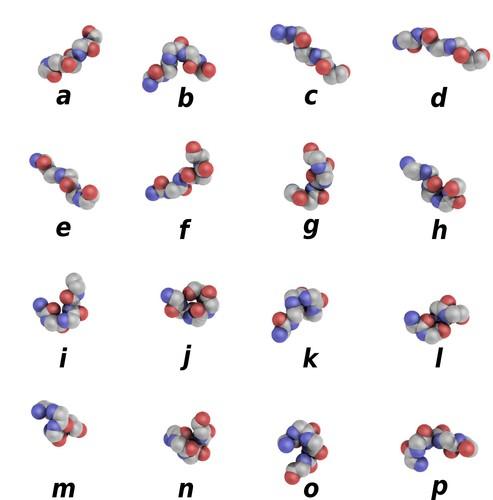
\includegraphics[width=0.7\textwidth]{./images/PBs.jpg}
    \caption{Šematski prikaz 16 proteinskih blokova označenh slovima od a do p}
    \label{Slika:1}
\end{figure}

Jedan od najpoznatijih strukturnih alfabeta jeste Proteinski blokovi (PB), koje je razvio De Brevern (2000). Proteinski blokovi se sastoji od 16 prototipova, koji su izdvojeni korišćenjem algoritama klasterovanja, Kohenonove samoorganizovajuće mape, nad fragmentima od pet uzastopnih aminokiselina kod proteina sa već poznatom strukturom. U prvom istraživanju je korišćeno 228 poznatih proteina, a kasnije je istraživanje ponovljeno nad 400 poznatih proteina. Procedura klasterovanja se odvijala u tri koraka. U prvom koraku se koristi mera sličnosti fragmenata RMSDA (eng. Root Mean Square Deviation on Angle), u drugom koraku se dodatno koristi i verovatnoća prelaska jednog fragmenta u drugi u sekvenci, dok se u trećem koraku izbacuje ograničenje verovatnoće prelaska. Na kraju je odabrano 16 proteinskih blokova, definisanih sa osam diedarskih uglova 8 diedarskih uglova, $\psi_{i-2}$, $\phi_{i-1}$, $\psi_{i-1}$, $\phi_i$, $\psi_i$, $\phi_{i+1}$, $\psi_{i+1}$, $\phi_{i+2}$ u odnosu na centralnu aminokiselinu u fragmentu dužine pet. (Tabela 1)
\\
\begin{table}[h!]
    \centering
    \begin{tabular}{|c|c|c|c|c|c|c|c|c|}
        \hline
        \textbf{PB} & \textbf{$\psi_{i-2}$} & \textbf{$\phi_{i-1}$} & \textbf{$\psi_{i-1}$} & \textbf{$\phi_i$} & \textbf{$\psi_i$} & \textbf{$\phi_{i+1}$} & \textbf{$\psi_{i+1}$} & \textbf{$\phi_{i+2}$ } \\
        \hline
        a & 41.14 & 75.53 & 13.92 & -99.80 & 131.88 & -96.27 & 122.08 & -99.68 \\ \hline
        b & 108.24 & -90.12 & 119.54 & -92.21 & -18.06 & -128.93 & 147.04 & -99.90 \\ \hline
        c & -11.61 & -105.66 & 94.81 & -106.09 & 133.56 & -106.93 & 135.97 & -100.63 \\ \hline
        d & 141.98 & -112.79 & 132.20 & -114.79 & 140.11 & -111.05 & 139.54 & -103.16 \\ \hline
        e & 133.25 & -112.37 & 137.64 & -108.13 & 133.00 & -87.30 & 120.54 & 77.40 \\ \hline
        f & 116.40 & -105.53 & 129.32 & -96.68 & 140.72 & -74.19 & -26.65 & -94.51 \\ \hline
        g & 0.40   & -81.83 & 4.91 & -100.59 & 85.50 & -71.65 & 130.78 & 84.98 \\ \hline
        h & 119.14 & -102.58 & 130.83 & -67.91 & 121.55 & 76.25 & -2.95 & -99.88 \\ \hline
        i & 130.68 & -56.92 & 119.26 & 77.85 & 10.42 & -99.43 & 141.40 & -98.01 \\ \hline
        j & 114.32 & -121.47 & 118.14 & 82.88 & -150.05 & -83.81 & 23.35 & -85.82 \\ \hline
        k & 117.16 & -95.41 & 140.40 & -59.35 & -29.23 & -72.39 & -25.08 & -76.16 \\ \hline
        l & 139.20 & -55.96 & -32.70 & -68.51 & -26.09 & -74.44 & -22.60 & -71.74 \\ \hline
        m & -39.62 & -64.73 & -39.52 & -65.54 & -38.88 & -66.89 & -37.76 & -70.19 \\ \hline
        n & -35.34 & -65.03 & -38.12 & -66.34 & -29.51 & -89.10 & -2.91 & 77.90 \\ \hline
        o & -45.29 & -67.44 & -27.72 & -87.27 & 5.13 & 77.49 & 30.71 & -93.23 \\ \hline
        p & -27.09 & -86.14 & 0.30 & 59.85 & 21.51 & -96.30 & 132.67 & -92.91 \\ \hline
    \end{tabular}
	\caption{Referentni uglovi Proteinskih blokova}
	\label{Tabela:1}
\end{table}

Proteinski blokovi su označeni slovima od a do p (Slika~\ref{Slika:1}). Najčešći proteinski blokovi, m i d, odgovaraju redom alfa-heliksu i beta-ravni. Proteinski blokovi od k do j odgovaraju nespecificnim strukturama (eng. coil).

Prevođenje u sekvencu proteinskih blokova kod proteina sa poznatom 3D strukturom odvija se tako što se svakom fragmentu uzastopnih aminokselina dužine pet dodeli jedan proteinski blok sa najmanjom vrednošću RMSDA-a. Može se desiti i da se diedralni uglovi ne mogu izračunati u tom se slučaju dodeljuje slovo Z. Na ovaj način svaka amino kiselina učestvuje u pet proteinskih blokova, osim prve i poslednje.

Strukturni alfabet Proteinski blokovi se koristi i u drugim podoblastima bioinformatike kao što su nadređivanje 3D strukture proteina, istraživanje strukture proteina, definisanje mesta vezivanja, i analize lokalnih konformacija poremećenih proteina.

Postoje alati koji prevode PDB fajlove u sekvence proteinskih blokova, kao što je Plxplore.

\newpage
\section{Analiza}
U ovom poglavlju analizirani su prelazi između proteinskih blokova. Fokus analize bio je na identifikaciji neočekivanih prelaza između proteinskih blokova i proučavanju aminokiselina i sekundarnim struktura prisutnih u njima. Dodatno, ispitane su vrednosti relevantnih parametara, kao i zastupljenost pojedinačnih aminokiselina u podacima.

\subsection{Opis podataka}
Podaci korišćeni u analizi obuhvataju informacije o proteinskim blokovima (PBs), aminokiselinama (AA), sekundarnim strukturama (S2), predviđenoj učestalosti prelaza, kao i dodatnim parametrima poput pLDDT i RSA. Izvor podataka su rezultati generisani pomoću AlphaFold2 programa. Konkretno, analiza je sprovedena nad dve datoteke: prvobitnog, obimnijeg skupa podataka, koji detaljnije opisuje prelaze između proteinskih blokova i manjeg podskupa dobijenog filtriranjem rezultata u skladu sa humanim proteomom. \\
Podaci su organizovani u tabelarnom formatu, pri čemu svaki red sadrži parove proteinskih blokova koji čine prelaz, parove aminokiselina i sekundarnih struktura koji ga opisuju, predviđenu učestalost prelaza i vrednosti parametara pLDDT i RSA.
\\
U nastavku je dat detaljan opis atributa:

\begin{itemize}
    \item \textbf{Protein\_number} – diskretan, kategorijski i redni atribut koji označava pojedinačne proteine u skupu podataka.
    \item \textbf{res\_number} – diskretan, kategorijski i redni atribut koji označava poziciju aminokiselinskog ostatka unutar sekvence.
    \item \textbf{PB1, PB2} – diskretni, kategorijski i nominalni atributi koji predstavljaju oznake proteinskih blokova između kojih dolazi do prelaza.
    \item \textbf{AA1, AA2} – diskretni, kategorijski i nominalni atributi koji opisuju aminokiseline prisutne u prelazu. Postoji ukupno 20 različitih vrednosti za ove atribute, u skladu sa standardnim skupom aminokiselina koje grade proteine. U tabeli \ref{table:1} prikazane su odgovarajuće jednoslovne oznake za svaku aminokiselinu.
\begin{table}[h!]
    \centering
	\begin{tabular}{ |l|c| } 
	\hline
	\textbf{Aminokiselina} &  \textbf{Jednoslovna oznaka}\\
	\hline
	Alanin &	 A \\
	\hline
	Arginin 	& R 	\\
	\hline
	Asparagin &	N \\
	\hline
	Asparaginska kiselina & D \\
	\hline
	Cistein 	& C 	\\
	\hline
	Glutaminska kiselina & E \\
	\hline
	Glutamin & Q \\
	\hline
	Glicin & G \\
	\hline
	Histidin & H \\
	\hline
	Izoleucin & I \\
	\hline
	Leucin & L \\
	\hline
	Lizin &	K \\
	\hline
	Metionin & M \\
	\hline
	Fenilalanin & F \\
	\hline
	Prolin & P \\
	\hline
	Serin & S \\
	\hline
	Treonin 	& T \\
	\hline
	Triptofan & W \\
	\hline
	Tirozin 	& Y \\
	\hline
	Valin & V  \\
	\hline
	\end{tabular}
	\caption{Aminokiseline i njihove jednoslovne oznake korišćene kao vrednosti atributa AA1 i AA2.}
	\label{table:1}
\end{table}
\newpage
    \item \textbf{S2\_1, S2\_2} – diskretni, kategorijski i nominalni atributi koji predstavljaju sekundarne strukture prisutne u prelazu. Vrednosti ovih atributa određene su pomoću DSSP (\textit{Dictionary of Secondary Structure of Proteins}) programa. DSSP program se koristi za dodeljivanje jednog od osam stanja sekundarne strukture aminokiselinama tako što se identifikuju vodonične veze između amino i karboksilnih grupa glavnog lanca proteina. \\
U tabeli \ref{table:2} prikazane su oznake i odgovarajući tipovi sekundarne strukture~\cite{carter2003dsspcont}.
\\
\begin{table}[h!]
    \centering
    \begin{tabular}{ |c|l| } 
    \hline
    \textbf{Oznaka} & \textbf{Tip sekundarne strukture} \\
    \hline
    H & Alfa-heliks (\textit{$\alpha$-helix}) \\
    B & Beta-most (\textit{beta bridge}) \\
    E & Prošireni beta list (\textit{extended beta sheet}) \\
    G & 3(10)-heliks \\
    I & Pi-heliks (\textit{$\pi$-heliks}) \\
    T & Heliks okret (\textit{helix-turn}) \\
    S & Zavojnica (\textit{bend}) \\
    C & Nespecifična ili neorganizovana struktura (\textit{coil}) \\
    \hline
    \end{tabular}
    \caption{Sekundarne strukture proteina prema DSSP standardu, korišćene kao vrednosti atributa S2\_1 i S2\_2.}
    \label{table:2}
\end{table}
\newpage
    \item \textbf{expected\_frequency} - neprekidan, kvantitativan i razmerni atribut čija vrednost pripada intervalu [0,1] i označava očekivanu učestalost prelaza između proteinskih blokova.
    \item \textbf{plDDT, RSA1, RSA2} – neprekidni, kvantitativni i razmerni atributi čije su vrednosti u intervalu [0,100]. Parametar pLDDT procenjuje pouzdanost predikcije lokalne strukture proteina, dok RSA1 i RSA2 predstavljaju relativnu dostupnost aminokiselinskih ostataka rastvaraču.
\end{itemize}
\subsubsection{Izdvajanje retkih prelaza između proteinskih blokova u podacima}
Glavni zadatak analize bio je proučavanje prelaza između proteinskih blokova pri čemu je akcenat stavljen na neočekivane, retke prelaze. Takvi prelazi su, zbog svoje prirode, od posebnog interesa za istraživanje jer mogu doprineti novim saznanjima o nizu proteinskih blokova koji opisuje trodimenzionalnu strukturu proteina. \\
U ovom radu, retkim prelazom smatra se onaj koji se javlja u manje od $1\%$ slučajeva. 
\subsection{Izdvajanje parova aminokiselina prisutnih u neočekivanim prelazima}
U cilju pronalaženja potencijalnih korelacija između atributa, odnosno između parova aminokiselina vezanih za retki prelaz i proteinskih blokova koji formiraju prelaz, izvršeno je izdvajanje tih parova. Pored toga, izračunate su frekvencije svih parova, a zatim su izdvojeni oni najfrekventiniji. \\ 
S obzirom na to da se u podacima korišćenim za ovu analizu prelazi ne nadovezuju, posmatran je pojedinačno svaki prelaz i unutar njega određen svaki par aminokiselina. Važno je napomenuti da redosled aminokiselina u paru nije irelevantan, zbog čega se parovi aminokiselina (A1, A2) ne mogu smatrati identičnim parovima (A2, A1). Kako bi ova tvrdnja bila intuitivnija i jasnija, potrebno je prvo objasniti zašto je prelaz određen sa dve aminokiseline iako su proteinski blokovi sačinjeni od 5 uzastopnih aminokiselina. \\ 
Naime, prilikom dodeljivanja proteinskog bloka fragmentu od 5 aminokiselina, centralna aminokiselina igra ključnu ulogu  jer je ona ta koja efektivno definiše fragment i omogućava izračunavanje 8 diedarskih uglova $\psi_{i-2}$, $\phi_{i-1}$, $\psi_{i-1}$, $\phi_i$, $\psi_i$, $\phi_{i+1}$, $\psi_{i+1}$, $\phi_{i+2}$.  Ovi uglovi se zatim upoređuju sa već definisanim diedarskim uglovima prototipova proteinskih blokova nakon čega se dodeljuje odgovarajući proteinski blok. Dakle, za svaki prelaz centralna aminokiselina je najvažnija zbog njenog uticaja na ceo fragment i zato je baš ona ta koja je izabrana da bude deo podataka, odnosno da bude predstavnik u prelazu. 

Imajući u vidu prethodno navedeno, obrnut redosled aminokiselina u paru može da predstavlja potpuno različit prelaz između proteinskih blokova i zato je važno analizirati ih kao zasebne parove. Slika \ref{fig:aa} prikazuje primer iz skupa podataka koji ilustruje iznesenu tvrdnju.
%\begin{figure}[htbp]
%    \centering
%    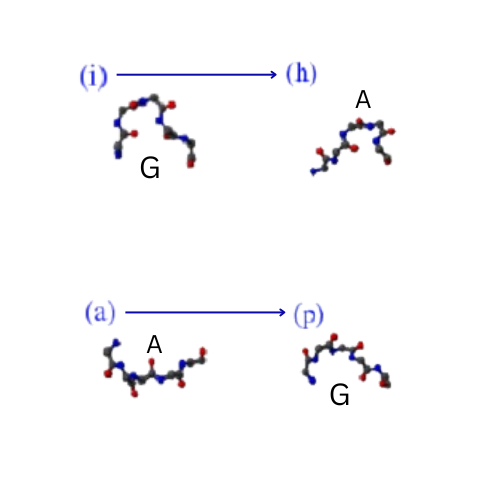
\includegraphics[width=0.5\textwidth]{/home/djurdja/Downloads/aa.png}
%    \caption{Redosled aminokiselina u paru je važan.}
%    \label{fig:aa}
%\end{figure}
\\
Izračunate su frekvencije svakog para aminokiselina u prelazima. Najčešće se javlja par (G, G). Pregled ostalih 19 najučestalijih parova dat je na slici \ref{fig:aafreq}.
%\begin{figure}[htbp]
%    \centering
%    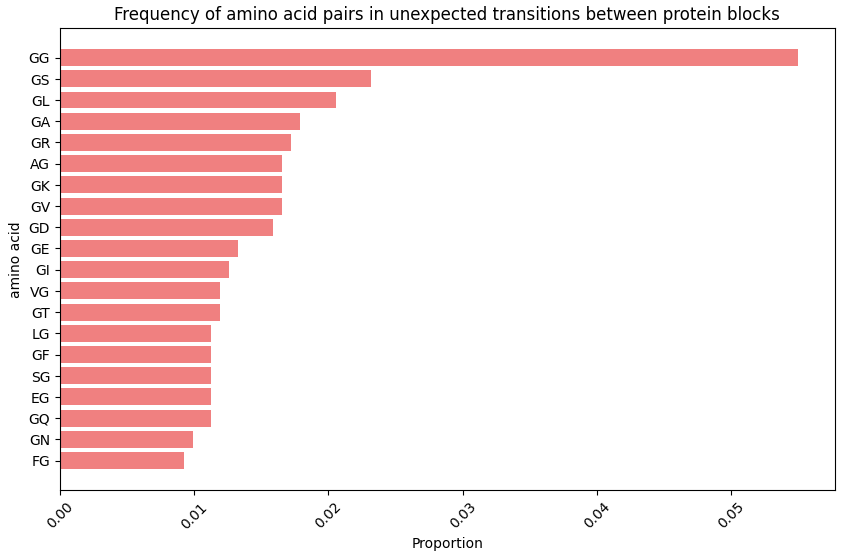
\includegraphics[width=1\textwidth]{/home/djurdja/Pictures/Screenshots/aafreq.png}
%    \caption{Frekvencija parova aminokiselina u retkim prelazima.}
%    \label{fig:aafreq}
%\end{figure}
\newpage
Dobijeni najfrekventniji par je od posebnog interesa s obzirom na specifične karakteristike glicina. Glicin ima najvažniju ulogu u formiranju sekundarne strukture alfa heliksa zahvaljujući svojoj fleksibilnosti, koja je rezultat izuzetno malog bočnog lanca. Takođe, glicin doprinosi stabilnosti tercijalne strukture proteina \cite{dong2015glycines}. Na osnovu ovoga, može se zaključiti da se u većini retkih prelaza postiže strukturna stabilnost zahvaljujući prisustvu glicina.
\subsection{Izdvajanje parova sekundarnih struktura koji se javljaju u neočekivanim prelazima}
\subsection{Analiza vrednosti pLDDT parametra}
\subsection{Analiza vrednosti RSA parametra}
\subsection{Ispitivanje zastupljenosti aminokiselina u podacima}
\newpage
\section{Klasifikacija}
\newpage
\section{Klasterovanje}
\newpage
\section{Zaključak}
\newpage
\begin{thebibliography}{5}
    \bibitem{carter2003dsspcont} 
    Phil Carter, Claus A. F. Andersen, Burkhard Rost. 
    \textit{DSSPcont: Continuous Secondary Structure Assignments for Proteins}. 
    Bioinformatics, 19(2):230-231, 2003.
    \bibitem{dong2015glycines} 
    Hao Dong, Mukesh Sharma, Huan-Xiang Zhou, Timothy A Cross. 
    \textit{Glycines: Role in $\alpha$-Helical Membrane Protein Structures and a Potential Indicator for Native Conformation}. 
    Biophysical Journal, 109(1):1-8, 2015.
\end{thebibliography}
\end{document}